%%%%% Preamble %%%%%
\documentclass[a4paper,11pt]{report}
\author{Walter Mottinelli e Andrea Bo}
\title{Trasformata $z$ e disposizione di poli e zeri\\ nei filtri FIR e IIR}
\usepackage{latexsym}
%\usepackage{makeidx} % to generate indexes
%\makeindex
\usepackage[italian]{babel}
\usepackage{ucs} % unicode encoding
\usepackage[utf8]{inputenc}
\usepackage{graphicx} % eps importing
\pagestyle{headings}
%\usepackage{fancyhdr}
%\pagestyle{fanccy}
%%%%%%%%%%%%%%%%%%%%
                                                                           
\begin{document}
\maketitle
\tableofcontents
\begin{abstract}
In questo documento viene presentata la trasformata $z$ e la disposizione di poli e zeri nel piano complesso. In relazione all'analisi numerica dei segnali, viene mostrata la correlazione tra il grafico poli/zeri di una funzione di trasferimento di un filtro e la risposta all'impulso dello stesso, con alcuni esempi di filtri FIR e IIR di uso comune.\\
Gli esempi e le illustrazioni che accompagnano la trattazione sono realizzati in Scilab, un applicativo free per il calcolo numerico.
\end{abstract}
\newcommand{\Figdir}{images/}
%%%%% Preamble %%%%%
%\documentclass[a4paper,11pt]{article}
%\author{Walter Mottinelli}
%\title{Elaborazione numerica dei segnali con Scilab}
%\usepackage{latexsym}
%\usepackage{makeidx} % to generate indexes
%\usepackage[italian]{babel}
%\usepackage{ucs} % unicode encoding
%\usepackage[utf8]{inputenc}
%\usepackage{graphicx} % eps importing
%\pagestyle{headings}
%%%%%%%%%%%%%%%%%%%%
                                                                           
%\begin{document}
%\maketitle
%\tableofcontents
%\begin{abstract}
%\end{abstract}

\chapter{La trasformata $z$}
La trasformata $z$ \`e uno dei principali strumenti matematici per l'analisi e la sintesi di filtri digitali. Trova infatti applicazione in alcune importanti problematiche, ad esempio:
\begin{itemize}
\item \emph{Calcolo della funzione di trasferimento del sistema} \\
La funzione di trasferimento di un filtro \`e la trasformata $z$ della sua risposta all'impulso. \\
Il piano complesso $z$ \`e utilizzato per mostrare la configurazione dei poli e degli zeri della funzione di trasferimento: la loro disposizione, come vedremo, \`e indice di importanti propriet\`a del sistema.\\
Inoltre, i coefficienti del filtro digitale possono essere ricavati direttamente a partire dalla funzione di trasferimento.
\item \emph{Calcolo delle trasformate di Fourier} \\
La trasformata di Fourier corrisponde al calcolo della trasformata $z$ lungo la circonferenza di raggio unitario con centro nell'origine degli assi del piano complesso $z$. In particolare, la versione discreta delle trasformata di Fourier viene valutata su insiemi di punti equidistanti tra loro.
\end{itemize}
\section{Definizione matematica}
La trasformata $z$ di una sequenza $\{h[n]\}$ \`e definita dalla funzione nella variabile $z$ a valori complessi
\begin{displaymath}
H(z) = \sum_{n=-\infty}^\infty h(n)z^{-n}
\end{displaymath}
e dalla regione di convergenza, luogo dei punti in cui la sommatoria \`e finita. \\
Se la sequenza $\{h[n]\}$ in esame \`e la risposta all'impulso di un filtro digitale, $H(n)$ viene chiamata \emph{funzione di trasferimento del sistema}.
\subsection*{Esempio di calcolo della trasformata $z$}
Sia data la funzione
\begin{displaymath}
h(n)=r^n cos(\omega_0 n)
\end{displaymath}
per $n\ge 0$, la cui trasformata $z$ \`e uguale a 
\begin{displaymath}
H(z)=\sum_{n=0}^\infty r^n cos(\omega_0 n)z^{-n}
\end{displaymath}
Applicando la formula
\begin{displaymath}
cos \omega = \frac{e^{i\omega n} + e^{-i\omega n}}{2}
\end{displaymath}
derivata dall'identit\`a di Eulero $e^{i\omega}=cos\omega + isen\omega$ 
e la formula della somma infinita di elementi di una serie geometrica\\
$\sum_{n=0}^\infty a^n = \frac{1}{1-a}$ per $|a|<1$ \\
otteniamo:
\begin{eqnarray*}
H(z) & = & \sum_{n=0}^\infty r^{n} \frac{e^{i\omega_0 n}+e^{-i\omega_0 n}}{2}z^{-n}\\
     & = & \frac{1}{2} \left [ \sum_{n=0}^\infty (re^{i\omega_0 n}z^{-1})^n + \sum_{n=0}^\infty (re^{-i\omega_0 n}z^{-1})^n\right ] \\
     & = & \frac{1}{2} \left [ \frac{1}{1-re^{i \omega_0}z^{-1}} + \frac{1}{1-re^{-i \omega_0}z^{-1}} \right ]\\
     & = & \frac{1}{2} \left [ \frac{2-r(e^{i\omega_0}+e^{-i\omega_0}z^{-1})}{(1-re^{i \omega_0}z^{-1})(1-re^{-i \omega_0})z^{-1}} \right ] \\
     & = & \frac{1-rcos(\omega_0)z^{-1}}{1-2rcos(\omega_0)z^{-1}+r^2 z^{-2}}
\end{eqnarray*}

\section{Propriet\`a della trasformata $z$}
\begin{itemize}
\item linearit\`a\\ se $\{x(n)\}=\{ah_1(n)+bh_2(n)\}$, allora $X(z)=aH_1(z)+bH_2(z)$
\item traslazione\\ se $\{y(n)\}=\{x(n-n_0)\}$, allora $Y(z)=z^{-n_0}X(z)$
\item convoluzione\\ se $\{y(n)\}=\{h(n)\}\ast\{x(n)\}$, allora $Y(z)=H(z)X(z)$
\item scalatura (nel dominio $z$)\\ se $\{y(n)\}=\{a^n x(n)\}$, allora $Y(z)=X(a^{-1} z)$
\item derivazione (nel dominio $z$)\\ se $\{y(n)\}=\{nx(n)\}$, allora $Y(z)=z^{-1} \frac{dX}{dz^{-1}}$
\end{itemize}

\section{Trasformate $z$ comuni}
\begin{tabular}{l|l|l}

Segnale & Trasformata $z$ & ROC \\
\hline
$\delta [n]$ & $1$ & $\forall z$ \\
$\delta [n-k]$ & $z^{-k}$ & $\forall z$, con $z\ne 0$ se $k>0$ \\
$\delta [n-k]$ & $z^{-k}$ & $\forall z$, con $z\ne \infty$ se $k<0$ \\
$u[n]$ & $\frac{z}{z-1}$ & $|z| > 1$ \\ 
$-(u[-n-1])$ & $\frac{z}{z-1}$ & $|z| < 1$ \\
$nu[n]$ & $\frac{z}{(z-1)^2}$ & $|z| > 1$ \\
$n^2 u[n]$ & $\frac{z(z+1)}{(z-1)^3}$ & $|z| > 1$ \\
$n^3 u[n]$ & $\frac{z(z^2 +4z +1)}{(z-1)^4}$ & $|z| > 1$ \\
$\left ( -\left(\alpha^n\right ) \right)u[-n-1]$ & $\frac{z}{z-\alpha}$ & $|z|<|\alpha|$ \\
$\alpha^n u[n]$ & $\frac{z}{z-\alpha}$ & $|z|>|\alpha|$ \\
$n\alpha^n u[n]$ & $\frac{\alpha z}{(z-\alpha)^2}$ & $|z|>|\alpha|$ \\
$n^2\alpha^n u[n]$ & $\frac{\alpha z(z+\alpha)}{(z-\alpha)^3}$ & $|z|>|\alpha|$ \\
$\frac{\prod_{k=1}^m (n-k+1)}{\alpha^m m!}\alpha^n u[n]$ & $\frac{z}{(z-\alpha)^{m+1}}$ \\
$\gamma^n cos(\alpha n)u[n]$ & $\frac{z(z-\gamma cos(\alpha))}{z^2 - (2\gamma cos(\alpha))z+\gamma^2}$ & $|z|>|\alpha|$ \\
$\gamma^n sen(\alpha n)u[n]$ & $\frac{z\gamma sen(\alpha)}{z^2 - (2\gamma cos(\alpha))z+\gamma^2}$ & $|z|>|\alpha|$
\end{tabular}

\section{Poli e zeri}
La trasformata $H(z)$ \`e una funzione nella variabile a valori complessi $z$, che pu\`o essere rappresentanta su un piano con la parte reale sull'asse delle ascisse e la parte immaginaria sull'asse delle ordinate.
Alcuni punti del piano complesso hanno particolare importanza:
\begin{itemize}
\item gli \emph{zeri} sono i punti in cui $H(z)=0$ 
\item i \emph{poli} sono i punti in cui $H(z)=\infty$
\end{itemize}
Con un grafico tridimensionale \`e possibile evidenziare il comportamento della trasformata in questi punti: in figura \ref{pole-zero-3D} \`e rappresentato in funzione di $\Re(z)$ e $\Im(z)$ il modulo di $H(z)=z^{-1}-1$, che ha uno zero in $z=1$ (l'avvallamento) e un polo in $z=0$ (il picco).
\input{images/pole-zero-3D.tex}
\dessin{Modulo di $H(z)=z^{-1}-1$ in funzione di $\Re(z)$ e $\Im(z)$}{pole-zero-3D}

Poli e zeri possono essere indicati esplicitamente nell'equazione di $H(z)$: consideriamo ad esempio una funzione di trasferimento di un segnale digitale, normalmente rappresentata come rapporto di somme di prodotti
\begin{displaymath}
H(z)=\frac{\sum_{k=-N_F}^{N_P} {b_k}z^{-k}} {1-\sum_{k=1}^Ma_kz^{-k}}
\end{displaymath}
dove 
\begin{itemize}
\item $N_F$ \`e il numero dei campioni in input successivi a quello in esame;
\item $N_P$ \`e il numero dei campioni in input precedenti quello in esame;
\item $M$  \`e il numero dei campioni in output precedenti quello in esame.
\end{itemize}
A partire da questa equazione \`e possibile passare ad un rapporto di prodotti di termini 
\begin{displaymath}
H(z)=Az^{N_F} \frac{\prod_{k=1}^{N_P+N_F}(1-c_k z^{-1})}{\prod_{k=1}^M (1-d_k z^{-1})}
\end{displaymath}
dove 
\begin{itemize}
\item A \`e una costante reale;
\item $c_k$, per $1\leq k \leq N_P + N_F$, \`e il valore (eventualmente complesso) del $k-esimo$ zero;
\item $d_k$, per $1\leq k \leq M$, \`e il valore del $k-esimo$ polo.
\end{itemize}
Alcune considerazioni sulla seconda rappresentazione:
\begin{itemize}
\item ogni fattore del numeratore ($1-c_kz^{-1}$) genera uno zero in $z=c_k$ e un polo in $z=0$;
\item ogni fattore del denominatore genera un polo in $z=d_k$ e uno zero in $z=0$;
\item nel punto $z=0$, poli dei fattori del numeratore cancellano zeri dei fattori del denominatore;
\item considerando anche i punti di singolarit\`a in $z=\infty$, il numero dei poli \`e \emph{sempre} pari al numero degli zero.
\end{itemize}
In sintesi, la disposizione dei poli e degli zeri della trasformata $z$ data nella forma 
\begin{displaymath}
H(z)=Az^{N_F} \frac{\prod_{k=1}^{N_P+N_F}(1-c_k z^{-1})}{\prod_{k=1}^M (1-d_k z^{-1)}}
\end{displaymath}
\`e la seguente:
\begin{itemize}
\item zeri in:
\begin{itemize}
\item $z=c_k$ \qquad per $1\leq k \leq N_P + N_F$
\item $z=0\textrm{ }$ \qquad di molteplicit\`a $M$
\item $z=0\textrm{ }$ \qquad di molteplicit\`a $N_F$
\end{itemize}
\item poli in:
\begin{itemize}
\item $z=d_k$ \qquad per $1\leq k \leq M$
\item $z=0\textrm{ }$ \qquad di molteplicit\`a $N_P + N_F$
\item $z=\infty$ \qquad di molteplicit\`a $N_F$
\end{itemize}
\end{itemize}

\subsection*{Esempio 1}
\begin{eqnarray*}
H(z) & = & \frac{1-rcos\left (\omega_0\right )z^{-1}}{1-2rcos{\omega_0}z^{-1}+r^2 z^{-2}} \\
     & = & \frac{1-rcos\left (\omega_0\right )z^{-1}}{1-r\left (e^{i\omega_0}+e^{-i\omega_0}\right )z^{-1}+r^2 z^{-2}} \\
     & = & \frac{1-rcos\left (\omega_0\right )z^{-1}}{\left (1-re^{i\omega_0}z^{-1}\right )\left (1-re^{-i\omega_0}z^{-1}\right )}
\end{eqnarray*}
Il numeratore genera uno zero in $z=rcos(\omega_0)$ e un polo in $z=0$, mentre il denominatore genera due zeri in $z=0$ e un polo in $z=re^{\pm i \omega_0}$.

\subsection*{Esempio 2 - singolarit\`a di second'ordine}
\begin{eqnarray*}
H(z) & = & z^2 + 2z + 3 + 2z^{-1} + z^{-2} \\
     & = & \left (z + 1 + z^{-1} \right )^2 \\
     & = & z^2 \left (1-c_1 z^{-1}\right )^2\left (1-c_2 z^{-1}\right )^2
\end{eqnarray*}
dove
\begin{eqnarray*}
c_1 & = & \frac{-1 + i\sqrt{3}}{2} = e^{-i2\pi/3} \\
c_2 & = & \frac{-1 - i\sqrt{3}}{2} = e^{-i2\pi/3}
\end{eqnarray*}
Il primo fattore genera due poli in $z=\infty$ e due zeri in $z=0$.
I due fattori contenenti $z^{-1}$ generano ciascuno due zeri in $z=c_1$ e $z=c_2$ e due poli in $z=0$.
\subsection*{Esempio 3 - zeri disposti sulla circonferenza unitaria}
$H(z)=1-z^{-N}$ \'e un polinomio di ordine N, e ha radici 
\begin{eqnarray*}
z^N & = & re^{i(\theta+2m \pi)/N} \\
    & = & r^{1/N}e^{i(\theta + 2m\pi)/N}
\end{eqnarray*}
dove $m$ \`e un intero.
Vale
\begin{displaymath}
z^N=1=e^{i2m\pi}
\end{displaymath} 
quindi gli zeri sono in $z=e^{(i2m\pi)/N}$, per $m=0, 1, 2, \ldots, N-1$: la loro posizione \`e lungo la circonferenza di raggio unitario e centro nell'origine degli assi, a partire da $z=1$ e distanziati di un angolo $2\pi/N$.
\section{La regione di convergenza (ROC)}
La trasformata $z$ \`e definita solo per valori di $z$ in cui $\sum_{n=-\infty}^\infty |h(n)z^{-n}|<\infty$. \\
Poich\'e $H(z)$ va all'infinito nei punti in cui sono definiti i poli, questi non possono trovarsi nella ROC. \\
Per individuare la ROC \`e possibile procedere nel seguente modo:
\begin{itemize}
\item per i segnali di durata finita, la ROC \`e l'intero piano Z escluso 
\begin{itemize}
\item $z=0$ per segnali causali
\item $z=\infty$ per segnali non causali
\item $z=0$ e  $z=\infty$ per i segnali bilaterali
\end{itemize}
\item per i segnali di durata infinita, la ROC \`e
\begin{itemize}
\item nel caso di segnali causali, l'intero piano eccetto il cerchio di raggio $r_1$ pari alla distanza tra l'origine e il polo finito pi\`u lontano
\item nel caso di segnali non causali, il cerchio di raggio $r_2$ pari alla distanza tra l'origine e il polo finito pi\`u vicino
\item nel caso di segnali bilaterali, l'anello racchiuso dalle circonferenze di raggio $r_1$ e $r_2$
\end{itemize}
\end{itemize}

La ROC \`e indispensabile per ottenere il segnale nel dominio temporale a partire dalla sua trasformata $z$, in quanto non vi \`e corrispondenza biunivoca tra un segnale e la sola forma analitica della sua trasformata $z$: segnali diversi possono avere la stessa trasformata, e quindi gli stessi poli e zeri, ma regione di convergenza diversa, come mostrato nel prossimo paragrafo.

\subsection{Determinazione della ROC di un segnale causale}
Prendiamo in considerazione il segnale
\begin{displaymath}
x(n)=a^n u(n)
\end{displaymath}
con
\begin{displaymath}
u(n)= \left\{
\begin{array}{ll}
1 & \textrm{per } n\geq0\\
0 & \textrm{altrimenti}
\end{array}
\right.
\end{displaymath}
cio\`e l'analogo discreto del segnale gradino unitario.\\
Calcolando la trasformata $z$ del segnale ${x(n)}$ si ricava
\begin{displaymath}
X(z) = \sum_{n=-\infty}^\infty a^{n}u(n)z^{-n}=\frac{1}{1-az^{-1}}=\frac{z}{z-a}
\end{displaymath}
Analizzando la trasformata $z$ si rileva uno zero in $z=0$ e un polo in $z=a$: la regione di convergenza \`e cos\`i definita per $|z|>|a|$, essendo il segnale causale.
Il diagramma poli/zeri pu\`o essere ottenuto con Scilab tramite i seguenti comandi:
\begin{verbatim}
// zero della funzione di trasferimento del filtro
a=.5;
// creazione del numeratore
Ncoeff=[0,1];
N=poly(Ncoeff,'z','coeff');
// creazione del denominatore
Dcoeff=[-(a),1];
D=poly(Dcoeff,'z','coeff');
// creazione della funzione di trasferimento H(z)=N/D
Ztrasf=syslin('d',N,D);
// disegno del grafico dei poli/zeri
xbasc(); xset("font size",4); plzr(Ztrasf);
// disegno della circonferenza che delimita la ROC (r=1)
xarc(-0.5,0.5,1,1,0,360*64)
\end{verbatim}
Come risultato otteniamo il grafico rappresentato in figura \ref{ROC_01}, in cui la ROC \`e stata evidenziata con una colorazione pi\`u scura.\\\\
\input{images/ROC_01.tex}
\dessin{Grafico della ROC e dei poli/zeri di un segnale causale}{ROC_01}

\subsection{Determinazione della ROC di un segnale non causale}
Prendiamo in considerazione il segnale
\begin{displaymath}
x(n)=-a^nu(-n-1)
\end{displaymath}
Calcolando la trasformata $z$ del segnale ${x(n)}$ si ricava
\begin{eqnarray*}
X(z) & = & -\sum_{n=-\infty}^\infty a^{n}u(-n-1)z^{-n} \\
     & = & -\sum_{n=-\infty}^{-1} a^{n}z^{-n} \\
     & = & 1-\sum_{n=0}^\infty (a^{1}z)^{-n} \\
     & = & \frac{z}{z-a}
\end{eqnarray*}
Analizzando la trasformata $z$ si rileva uno zero in $z=0$ e un polo in $z=a$: la regione di convergenza \`e definita per $|z|<|a|$, essendo il segnale non causale. \\
Il diagramma poli/zeri pu\`o essere ottenuto con Scilab tramite i seguenti comandi:
\begin{verbatim}
// zero della funzione di trasferimento del filtro
a=.5;
// creazione del numeratore
Ncoeff=[0,1];
N=poly(Ncoeff,'z','coeff');
// creazione del denominatore
Dcoeff=[-(a),1];
D=poly(Dcoeff,'z','coeff');
// creazione della funzione di trasferimento H(z)=N/D
Ztrasf=syslin('d',N,D);
// disegno del grafico dei poli/zeri
xbasc(); xset("font size",4); plzr(Ztrasf);
// disegno della circonferenza che delimita la ROC (r=1)
xarc(-0.5,0.5,1,1,0,360*64)
\end{verbatim}
Come risultato otteniamo il grafico rappresentato in figura \ref{ROC_02}, in cui la ROC \`e stata evidenziata con una colorazione pi\`u scura.
\input{images/ROC_02.tex}
\dessin{Grafico della ROC e dei poli/zeri di un segnale non causale}{ROC_02}

\subsection{Determinazione della ROC di un segnale bilatero}
Prendiamo in considerazione il segnale
\begin{displaymath}
x(n)=\left(-\frac{1}{4}\right)^{n}u(n)-\left(\frac{1}{2}\right)^{n}u(-n-1)
\end{displaymath}
Calcoliamo la trasformata $z$ del segnale ${x(n)}$ scomponendolo in due parti:
\begin{eqnarray*}
\left(-\frac{1}{4}\right)^nu(n) & \longrightarrow & \frac{z}{z+\frac{1}{4}} \\
-\left(\frac{1}{2}\right)^n u(n) & \longrightarrow & \frac{z}{z-\frac{1}{2}}
\end{eqnarray*}
quindi la trasformata $z$ finale risulta essere
\begin{displaymath}
X(z) = \frac{z}{z+\frac{1}{4}}+\frac{z}{z-\frac{1}{2}}=\frac{z(2z-\frac{1}{8})}{(z+\frac{1}{4})(z-\frac{1}{2})}
\end{displaymath}
Analizzando la trasformata $z$ si rilevano due zeri $\left( z=0 \textrm{ e } z=\frac{1}{16} \right)$ e due poli $\left( z=-\frac{1}{4} \textrm{ e } z=\frac{1}{2}\right)$.\\
Utilizzando la propriet\`a di linearit\`a della trasformata $z$ possiamo concludere che la regione di convergenza \`e definita come l'intersezione delle regioni di convergenza delle due parti del segnale, quindi \`e uguale a $\frac{1}{4}<|z|<\frac{1}{2}$.\\
Il diagramma dei poli-zeri pu\`o essere ottenuto con Scilab tramite i seguenti comandi:
\begin{verbatim}
// creazione del numeratore
Ncoeff=[0,-(1/8),2];
N=poly(Ncoeff,'z','coeff');
// creazione del denominatore
Dcoeff=[-(1/8),-(1/4),1];
D=poly(Dcoeff,'z','coeff');
// creazione della trasformata Z
Ztrasf=syslin('d',N,D)
// stampa del grafico
xbasc(); xset("font size",4); plzr(Ztrasf);
// disegno della circonferenza che delimita la ROC
xarc(-.5,.5,1,1,0,360*64)	// Anello esterno
xarc(-.25,.25,.5,.5,0,360*64)	// Anello interno
\end{verbatim}
Come risultato otteniamo il grafico rappresentato in figura \ref{ROC_03}, in cui la ROC \`e stata evidenziata con una colorazione pi\`u scura.\\
Il diagramma del modulo e della fase del filtro pu\`o essere ottenuto con Scilab tramite i seguenti comandi:
\begin{verbatim}
// creazione del numeratore
Ncoeff=[0,-(1/8),2];
N=poly(Ncoeff,'z','coeff');
// creazione del denominatore
Dcoeff=[-(1/8),-(1/4),1];
D=poly(Dcoeff,'z','coeff');
// range di frequenze
f=(0:.01:.5);
// calcolo della risposta in frequenza
hf=freq(N,D,exp(2*%pi*%i*f));
xbasc(); xset("font size",4);
xsetech([0,0,1,.5]); plot2d(f,(abs(hf)))
xtitle("Risposta in frequenza del filtro")
xsetech([0,.5,1,.5]); plot2d(f,atan(imag(hf),real(hf)));
xtitle("Risposta in fase del filtro")
\end{verbatim}
Come risultato otteniamo il grafico rappresentato in figura \ref{Grafico_MagFase_3}.\\\\
\input{images/ROC_03.tex}
\dessin{Grafico della ROC e dei poli/zeri di un segnale bilatero}{ROC_03}
\input{images/Grafico_MagFase_3.tex}
\dessin{Risposta in frequenza e in fase di un filtro bilatero}{Grafico_MagFase_3}

\section{Calcolo della trasformata inversa}
La trasformata $z$ inversa permette di tornare dal piano $z$ al dominio d'origine: esistono quattro principali metodi per il calcolo dell'antitrasformata.
\subsection{Metodo delle funzioni parziali}
Uno dei metodi pi\`u semplici, e al tempo stesso pi\`u utili, per calcolare l'antitrasformata $z$ consiste nel decomporre la trasformata in frazioni parziali.
Consideriamo ad esempio la trasformata
\begin{displaymath}
X(z)=\frac{1}{1-\frac{3}{2}z^{-1}+\frac{1}{2}z^{-2}}
\end{displaymath}
Fattorizziamo il denominatore in modo da ottenere
\begin{displaymath}
X(z)=\frac{1}{(1-z^{-1})(1-\frac{1}{2}z^{-1})}
\end{displaymath}
$X(z)$ pu\`o quindi essere espressa come 
\begin{displaymath}
X(z)=\frac{A}{1-z^{-1}}+\frac{B}{1-\frac{1}{2}z^{-1}}
\end{displaymath}
con $A=2$ e $B=-1$.\\
Grazie alla propriet\`a di linearit\`a, le due frazioni possono essere invertite separatamente: sono due trasformate semplici (presenti nella tabella delle trasformata pi\`u comuni), quindi otteniamo
\begin{displaymath}
x(n)=Z^{-1}{X(z)}=2u(n)-\left ({\frac{1}{2}}\right )^n u(n)
\end{displaymath}
\subsection{Metodo della divisione}
A partire dalla funzione di trasferimento espressa come rapporto tra numeratore e denominatore, \`e possibile eseguire la divisione polinomiale ed ottenere quindi un unico polinomio: la sua trasformata inversa \`e una successione di impulsi pesati.
Riprendiamo l'esempio precedente: 
\begin{displaymath}
X(z)=\frac{1}{1-\frac{3}{2}z^{-1}+\frac{1}{2}z^{-2}}
\end{displaymath}
Effettuando la divisione si ottiene:
\begin{displaymath}
X(z)=1+ \frac{3}{2} z^{-1}+ \frac{7}{4} z^{-2}+ + \frac{15}{8} z^{-3} +\ldots
\end{displaymath}
la cui trasformata inversa \`e
\begin{displaymath}
x(n)=\delta(n)+ \frac{3}{2}\delta(n-1)+ \frac{7}{4}\delta(n-2)+ \frac{15}{8}\delta(n-3) + \ldots
\end{displaymath}

\subsection{Metodo del prodotto di Cauchy}
Analogamente al precedente, questo metodo consente di ottenere la trasformata inversa come somma di impulsi pesati e ritardati nel tempo.
Se $X(z)$ \`e nella forma
\begin{displaymath}
X(z)=\frac{b_0 + b_1 z^{-1}+\ldots + b_m z^{-m}}{a_0 + a_1 z^{-1}+\ldots + a_m z^{-m}}
\end{displaymath}
applicando il prodotto di Cauchy (il prodotto di convoluzione) e manipolando l'equazione in x(n) si ottiene l'equazione ricorsiva
\begin{displaymath}
x(n)=\frac{1}{a_0}\left[ b_n - \sum_{k=0}^{n-1} x(k) a_{n-k}\right]
\end{displaymath}
con $a_0 \neq 0$. \\
Nell'esempio precedente
\begin{displaymath}
X(z)=\frac{1}{1-\frac{3}{2}z^{-1}+\frac{1}{2}z^{-2}}
\end{displaymath}
i pesi sono
\begin{displaymath}
b_0 = 1, a_0=1, a_1=-\frac{3}{2}, a_2=\frac{1}{2}
\end{displaymath}
\`E possibile applicare l'equazione ricorsiva in x(n) e ottenere
\begin{displaymath}
x(0)=1, x(1)=\frac{3}{2}, x(2)=\frac{7}{4}, x(3)=\frac{15}{8}, \ldots
\end{displaymath}

\subsection{Metodo di integrazione}
Questo metodo \`e analiticamente il pi\`u complicato. \`E possibile dimostrare che esiste una relazione diretta tra l'$n-esimo$ elemento di una sequenza a tempo discreto ${h(n)}$ e la sua trasformata $z$, secondo la relazione:
\begin{displaymath}
x(n)=\frac{1}{2\pi i}\oint_C X(z)z^{n-1}dz
\end{displaymath}
dove l'integrazione \`e eseguita in senso antiorario lungo un percorso chiuso racchiudente l'origine degli assi ed interamente contenuto nella ROC.\\
Il calcolo diretto dell'integrale \`e spesso difficile, quindi viene utilizzato un secondo risultato, il \emph{teorema dei residui}:
\begin{displaymath}
h(n)=\sum_{i=1}^{N} \textrm{Res}[H(z)z^{n-1} \textrm{ nel polo }p_i]
\end{displaymath}
dove $\textrm{Res}[\cdot]$ \`e il \emph{residuo}.
Per definire il residuo, sia $H(z)z^{n-1}$ una funzione razionale in $z$ con un polo di ordine $m$ in $z=z_0$:
\begin{displaymath}
H(z)z^{n-1}=\frac{P(z)}{(z-z_0)^m}
\end{displaymath}
Il residuo di $H(z)z^{n-1}$ in $z=z_0$ \`e definito come
\begin{displaymath}
\textrm{Res}[H(z)z^{n-1} \textrm{ nel polo }p_i]=\left. \frac{1}{(m-1)!}\frac{d^{m-1}P(z)}{dz^{m-1}}\right |_{z=z_0}
\end{displaymath}

%%%%% Preamble %%%%%
%\documentclass[a4paper,11pt]{article}
%\author{Walter Mottinelli}
%\title{Elaborazione numerica dei segnali con Scilab}
%\usepackage{latexsym}
%\usepackage{makeidx} % to generate indexes
%\usepackage[italian]{babel}
%\usepackage{ucs} % unicode encoding
%\usepackage[utf8]{inputenc}
%\usepackage{graphicx} % eps importing
%\pagestyle{headings}
%%%%%%%%%%%%%%%%%%%%
                                                                           
%\begin{document}
%\maketitle
%\tableofcontents
%\begin{abstract}
%\end{abstract}

\chapter{Trasformata $z$ e filtri digitali}
\section{Calcolo della funzione di trasferimento\ldots}
Nel dominio $z$, un sistema si comporta secondo la sua \emph{funzione di trasferimento}, cio\`e la trasformata $z$ della sua risposta all'impulso, quindi \`e importante poterla calcolare a partire dalle sequenze di ingresso e uscita o dalla equazione alle differenze.
\subsection*{\ldots\textrm{} date le sequenze di ingresso e di uscita}
Consideriamo ad esempio il filtro che converte la sequenza di ingresso
\begin{displaymath}
x(n)=r^n cos(\omega_0 n)
\end{displaymath}
(per $n \geq 0$) in \\
\begin{displaymath}
y(n)=r^n sen(\omega_0 n)
\end{displaymath}
(per $n \geq 0)$ e le loro trasformate \\
\begin{eqnarray*}
X(Z) & = & \frac{1-rcos(\omega_0)z^{-1}}{1-2rcos(\omega_0)z^{-1}r^2 z^{-2}} \\ 
Y(Z) & = & \frac{rsen(\omega_0)z^{-1}}{1-2rcos(\omega_0)z^{-1}r^2 z^{-2}}
\end{eqnarray*}
La funzione di trasferimento richiesta \`e data da 
\begin{eqnarray*}
H(z) & = & Y(z)/X(z) \\
     & = & \frac{rsen(\omega_0)z^{-1}}{1-rcos(\omega_0)z^{-1}}
\end{eqnarray*}
\subsection*{\ldots\textrm{} data l'equazione alle differenze}
Un sistema lineare tempo-invariante \`e descritto dalla seguente equazione alle differenze
\begin{displaymath}
y(n)=\sum_{k=1}^M a_k y(n-k) + \sum_{k=-N_F}^{N_P}b_k x(n-k)
\end{displaymath}
Prendiamone la trasformata $z$ e riordiniamone le sommatorie:
\begin{eqnarray*}
Y(z) & = & \sum_{n=-\infty}^{\infty} y(n)z^{-n} \\
     & = & \sum_{n=-\infty}^{\infty} \left [ \sum_{k=1}^M a_k y(n-k) + \sum_{k=-N_F}^{N_P} b_k x(n-k) \right] z^{-n} \\
     & = & \sum_{k=1}^M a_k \left [ \sum_{n=-\infty}^{\infty} y(n-k)z^{-n}\right ] + \sum_{k=-N_F}^{N_P} b_k \left [ \sum_{n=-\infty}^{\infty} x(n-k)z^{-n}\right ]
\end{eqnarray*}
Applicando la regola della trasformata $z$ di una sequenza ritardata, otteniamo
\begin{displaymath}
Y(z)=\sum_{k=1}^M a_k z^{-k}Y(z) + \sum_{k=-N_F}^{N_P} b_k z^{-k} X(z)
\end{displaymath}
Separiamo gli addendi contenenti $X(z)$ e $Y(z)$ e applichiamo la definizione della funzione di trasferimento $H(z)$: otteniamo il risultato atteso
\begin{displaymath}
H(z)=\frac{Y(z)}{X(z)}=\frac{\sum_{k=-{N_F}}^{N_P} b_k z^{-k}}{1- \sum_{k=1}^M a_k z^{-k}}
\end{displaymath}

\subsection*{Esempio di calcolo}
Consideriamo l'equazione alle differenze \\
\begin{displaymath}
y(n)=a_1 y(n-1)+a_2 y(n-2)+b_0 x(n)+b_1 x(n-1)
\end{displaymath}
Prendiamone la trasformata $z$
\begin{eqnarray*}
Y(z) & = & a_1z^{-1}Y(z)+a_2z^{-2}Y(z)+b_0 X(z)+b_1 z^{-1}X(z) \\
     & = & \frac{(b_0 + b_1 z^{-1})}{(1-a_1 z^{-1}-a_2 z^{-2})}X(z)
\end{eqnarray*}
La funzione di trasferimento \`e quindi 
\begin{displaymath}
H(z)=\frac{b_0 + b_1 z^{-1}}{1-a_1 z^{-1} -a_2 z^{-2}}
\end{displaymath}

\section{Disposizione di poli e zeri in un filtro generico}
Ricordiamo la scrittura della funzione di trasferimento come rapporto di due polinomi:
\begin{displaymath}
X(z)=\frac{P(z)}{Q(z)}
\end{displaymath}
Gli zeri, cio\`e i valori di $z$ per cui $P(z)=0$, indicano le frequenze complesse in cui il guadagno del filtro \`e nullo.
I poli, cio\`e i valori di $z$ per cui $Q(z)=0$, indicano le frequenze complesse in cui il guadagno del filtro \`e infinito.\\
Poli e zeri vicini all'origine non modificano significativamente la risposta in
frequenza del filtro, mentre zeri vicini alla circonferenza portano a zero le frequenze corrispondenti.\\
Se la ROC si estende oltre il polo pi\`u distante dal centro, allora il sistema \`e causale. Se la ROC include la circonferenza unitaria, allora il sistema \`e stabile. Ne segue che un filtro \`e causale e stabile se i poli sono tutti contenuti nel cerchio unitario.\\
Poich\'e ogni filtro pu\`o essere scomposto in filtri elementari di primo e secondo ordine, a loro volta distinguibili in ricorsivi e non ricorsivi, sono quattro le combinazioni base di poli e zeri:
\begin{itemize}
\item uno zero sull'asse reale in $z=r_0$ con $0 < r_0 < \infty$ e il polo corrispondente in $z=0$. La funzione di trasferimento del filtro non ricorsivo di prim'ordine che genera questa disposizione \`e 
\begin{displaymath}
H_1(z)=1-r_0 z^{-1}
\end{displaymath}
\item un polo sull'asse reale in posizione $z=r_0$ con $0 < r_0 < 1$ e il zero corrispondente in $z=0$. La funzione di trasferimento del filtro ricorsivo di prim'ordine che genera questa disposizione \`e 
\begin{displaymath}
H_2(z)=\left [1-r_0 z^{-1}\right ]^{-1}
\end{displaymath}
\item una coppia coniugata di zeri complessi in $z=r_0 e^{\pm i\omega_0}$ con $0 < r_0 < \infty$ e due poli corrispondenti in $z=0$. La funzione di trasferimento del filtro non ricorsivo di second'ordine che genera questa disposizione \`e 
\begin{displaymath}
H_3(z)=(1-r_0 e^{i\omega_0} z^{-1})(1-r_0 e^{-i\omega_0} z^{-1})=1-2r_0 cos(\omega_0)z^{-1}+r^2 z_0^{-2}
\end{displaymath}
\item una coppia coniugata di poli complessi in $z=r_0 e^{\pm i\omega_0}$ con $0 < r_0 < 1$ e due zeri corrispondenti in $z=0$. La funzione di trasferimento del filtro ricorsivo di second'ordine che genera questa disposizione \`e 
\begin{eqnarray*}
H_4(z) & = & \left[(1-r_0 e^{i\omega_0} z^{-1})(1-r_0 e^{-i\omega_0} z^{-1})\right ]^{-1} \\
       & = & \left[1-2r_0 cos(\omega_0)z^{-1}+r^2 z_0^{-2}\right]^{-1}
\end{eqnarray*}
\end{itemize}
In una funzione di trasferimento, gli zeri e i poli sono in numero uguale se vengono considerati anche i punti di singolarit\`a in $z=\infty$. Se, dopo aver analizzato i punti di singolarit\`a finiti, resta un disavanzo di $n$ zeri, significa che ci sono $n$ poli in $z=\infty$. La funzione di trasferimento di questa componente \`e 
\begin{displaymath}
H(5)=z^{n}
\end{displaymath}
ed \`e caratteristica dei sistemi non causali: la risposta all'impulso \`e anticipata di $n$ campioni. n caso di disavanzo di $n$ poli, si avranno $n$ zeri in $z=\infty$: la risposta all'impulso \`e ritardata di $n$ campioni.\\
La funzione di trasferimento complessiva di un filtro costituito da queste componenti \`e proporzionale al prodotto delle singole funzioni di trasferimento.

\subsection{Grafico della risposta in frequenza e in fase}

Mostriamo come poter ottenere con Scilab la risposta in frequenza e in fase di un filtro con funzione di trasferimento $H(z)=\frac{z}{z-a}$:

\begin{verbatim}
// zero della funzione di trasferimento del filtro
a=.5;
// creazione del numeratore
Ncoeff=[0,1];
N=poly(Ncoeff,'z','coeff');
// creazione del denominatore
Dcoeff=[-(a),1];
D=poly(Dcoeff,'z','coeff');
// definizione del range di frequenza
f=(0:.01:.5);
// calcolo della risposta in frequenza
hf=freq(N,D,exp(2*%pi*%i*f));
// settiamo la finestra per il grafico e lo visualizziamo
xbasc(); xset("font size",4);
xsetech([0,0,1,.5]); plot2d(f,(abs(hf)))
xtitle("Risposta in frequenza")
xsetech([0,.5,1,.5]); plot2d(f,atan(imag(hf),real(hf)));
xitle("Fase del filtro")
\end{verbatim}
Come risultato otteniamo il grafico rappresentato in figura \ref{Grafico_MagFase_1-2}.
\input{images/Grafico_MagFase_1-2.tex}
\dessin{Risposta in frequenza e in fase di $H(z)=\frac{z}{z-0,5}$}{Grafico_MagFase_1-2}
                                                                               
Al fine di evidenziare l'importanza del posizionamento degli zeri nel piano complesso $z$, riportiamo i grafici del modulo (figura \ref{Grafico_confronto_Mag}) e della fase (figura \ref{Grafico_confronto_Fase}) del filtro avente $H(z)=\frac{z}{z-a}$ per valori variabili dello zero $a$.
\input{images/Grafico_confronto_Mag.tex}
\dessin{Variazione della risposta in frequenza rispetto al valore dello zero (rosso=1.25; verde=0.75; blu=0.5; nero=0.25)}{Grafico_confronto_Mag}
\input{images/Grafico_confronto_Fase.tex}
\dessin{Variazione della fase rispetto al valore dello zero (rosso=1.25; verde=0.75; blu=0.5; nero=0.25)}{Grafico_confronto_Fase}


\section*{Disposizione di zeri e poli in un filtro a fase lineare}
Gli zeri di una funzione di trasferimento di un filtro lineare seguono una configurazione precisa.
Ricordando che un filtro \`e lineare se \`e simmetrico, scriviamo la stessa condizione nel dominio $Z$ e applichiamo la trasformata $z$:
\begin{eqnarray*}
h(n) & = & h(N-(1-n)) \\
H(z) & = & z^{-(N-1)H\left (\frac{1}{z}\right )}
\end{eqnarray*}
Ricordiamo che stiamo considerando un segnale ${h(n)}$ a valori reali: quindi, se $z_0$ \`e uno zero di $H(z)$, allora lo \`e anche il suo complesso coniugato $\bar{z_0}$; sfruttando la condizione di simmetria precedente, anche $\left (\frac{1}{z_0}\right )$ e $\left (\frac{1}{\bar{z_0}}\right )$ sono radici, quindi gli zeri generici di un filtro lineare esistono a gruppi di quattro.

\section{Progetto di filtri mediante disposizione \\iterativa di poli/zeri}
Lo scopo di questa sezione \`e di determinare la struttura di un filtro e dei suoi coefficienti posizionando in maniera iterativa poli e zeri nel piano $z$, osservando il risultato ottenuto dopo il loro posizionamento fino a quando non si realizza il filtro con le specifiche richieste.\\
Per semplificare la realizzazione del filtro si possono tener presente le seguenti regole e consigli:\\
\\
\emph{Regole}
\begin{itemize}
\item Le specifiche della risposta in frequenza consistono in regioni passa-banda e taglia-banda (vedi figura \ref{Prog-FiltroPB}). Queste bande sono mappate sulla circonferenza di raggio unitario con lo scopo di facilitare il posizionamento dei poli e degli zeri.
\item Tutti i poli dovranno avere un raggio $r_p$ compreso nell'intervallo \\$0,6\leq r_p<0,96$.\\
Il limite superiore garantisce che nella fase di realizzazione pratica eventuali errori di troncamento o arrotondamento causino l'instabilit\`a del filtro mentre il limite inferiore serve ad evitare di avere poli che diano una scarsa risposta in frequenza.
\item La progettazione del filtro viene ottimizzata analizzando, dopo ogni posizionamento di poli e zeri, il grafico della risposta in frequenza.\\
Operando in questo modo si pu\`o rimuovere la singolarit\`a o modificarne la posizione nel caso in cui non si ottenga l'effetto desiderato.
\end{itemize}
\emph{Consigli}
\begin{itemize}
\item Lo sviluppo dovrebbe iniziare posizionando un polo a distanza $r_p$ in mezzo ad ogni zona passa-banda e uno zero in mezzo ad ogni zona taglia-banda sulla circonferenza unitaria.
\item La risposta in frequenza al di sopra di una limitata banda di frequenze pu\`o essere incrementata inserendo, nella circonferenza di raggio unitario, un polo nell'angolo corrispondente al centro della banda interessata. La dimensione del raggio del polo determiner\`a l'aumento sia della banda sia del guadagno.
\item La risposta in frequenza al di sopra di una banda limitata pu\`o essere diminuita posizionando uno zero nell'angolo corrispondente al centro della banda. Per ottenere un'attenuazione massima, lo zero dovr\`a essere posizionato sulla circonferenza di raggio unitario.
\end{itemize}

\subsection{Realizzazione iterativa di un filtro passa-basso}
Proveremo ora a realizzare un filtro seguendo le indicazioni precedentemente citate.
Le caratteristiche del filtro passa-basso sono:\\
passa-banda
\begin{displaymath}
-1<|H(e^{j\omega})|_{dB}\leq0 \qquad\textrm{per } 0\leq\omega\leq\frac{\pi}{4}
\end{displaymath}
taglia-banda
\begin{displaymath}
|H(e^{j\omega})|_{dB}\leq-50 \qquad\textrm{per } \frac{\pi}{2}\leq\omega\leq\pi
\end{displaymath}

Le zone di interesse sono evidenziate nella figura \ref{Prog-FiltroPB}.\\
\begin{figure}[hp]
  \centering
  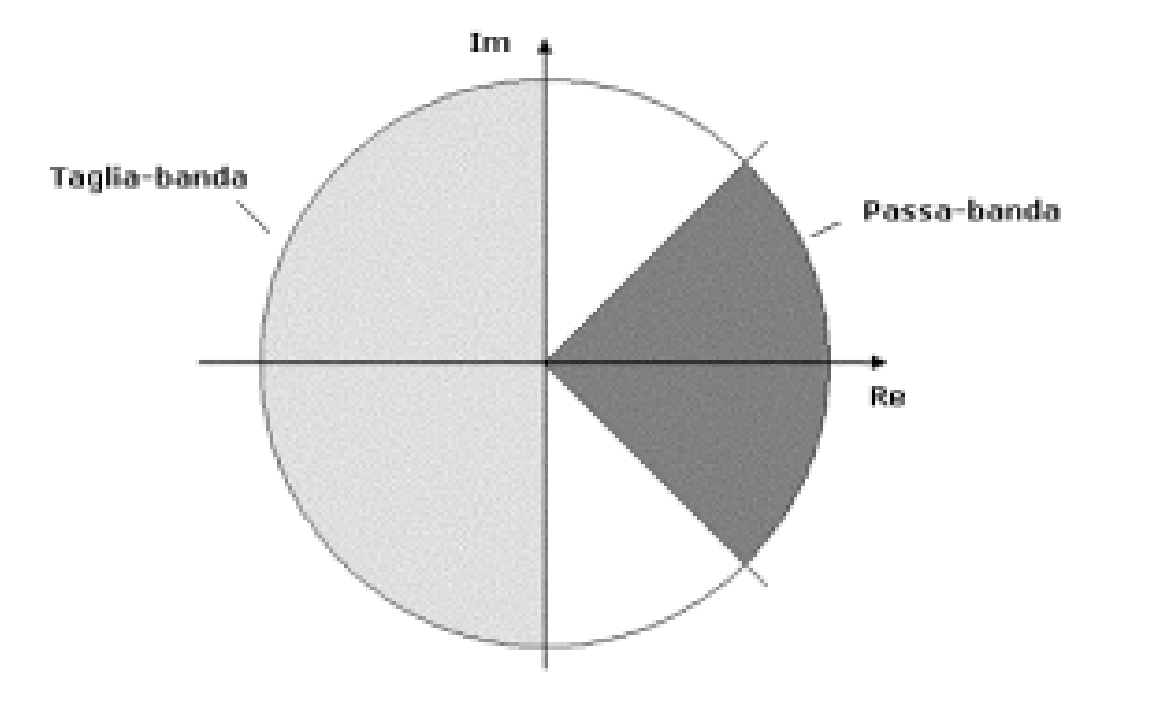
\includegraphics[scale=0.5]{images/Prog-FiltroPB.eps}
  \caption{Settori in cui verranno disposti i poli e gli zeri}
  \label{Prog-FiltroPB}
\end{figure}
%\input{images/Prog-FiltroPB.tex}
%\dessin{Settori in cui verranno disposti i poli e gli zeri}{Prog-FiltroPB}

\subsubsection*{Passi della realizzazione}
\begin{itemize}
\item \emph{Singolarit\`a 1 e 2}\\
Posizionare un polo con raggio $r=0.7$ in mezzo alla zona passa-banda e uno zero in mezzo alla zona taglia-banda, sulla circonferenza unitaria.\\
La funzione di trasferimento del filtro risulta
\begin{displaymath}
H(z)=\frac{1+z^{-1}}{1-0,7z^{-1}}
\end{displaymath}
Il grafico della risposta in frequenza del filtro \`e rappresentato in figura \ref{RispFreq-Hz_sing1-2}.
\input{images/RispFreq-Hz_sing1-2.tex}
\dessin{Risposta in frequenza del filtro dopo il posizionamento delle singolarit\`a 1 e 2}{RispFreq-Hz_sing1-2} 
\item \emph{Singolarit\`a 3} \\
Inserire uno zero in testa alla zona taglia-banda, sulla circonferenza unitaria.\\
La funzione di trasferimento del filtro risulta
\begin{displaymath}
H(z)=\frac{(1+z^{-1})(1+z^{-2})}{1-0,7z^{-1}}
\end{displaymath}
Il grafico della risposta in frequenza del filtro \`e rappresentato in figura \ref{RispFreq-Hz_sing3}.
\input{images/RispFreq-Hz_sing3.tex}
\dessin{Risposta in frequenza del filtro dopo il posizionamento della singolarit\`a 3}{RispFreq-Hz_sing3}

\item \emph{Singolarit\`a 4} \\
Aggiungere un polo a $z=0,9e^{\pm j50^{\circ}}$ per sollevare la risposta in frequenza nella zona passa-banda.\\
La funzione di trasferimento del filtro risulta
\begin{displaymath}
H(z)=\frac{(1+z^{-1})(1+z^{-2})}{(1-0,7z^{-1})(1-1,16z^{-1}+0,81z^{-2})}
\end{displaymath}
Il grafico della risposta in frequenza del filtro \`e rappresentato in figura \ref{RispFreq-Hz_sing4}.
\input{images/RispFreq-Hz_sing4.tex}
\dessin{Risposta in frequenza del filtro dopo il posizionamento della singolarit\`a 4}{RispFreq-Hz_sing4}

\item \emph{Singolarit\`a 5} \\
Posizionare uno zero sulla circonferenza unitaria, dove risulta massima la risposta nella zona taglia-banda. Questo zero limita l'incremento dovuto alla singolarit\`a 4.\\
La funzione di trasferimento del filtro risulta
\begin{displaymath}
H(z)=\frac{(1+z^{-1})(1+z^{-2})(1+1,03z^{-1}+z^{-2})}{(1-0,7z^{-1})(1-1,16z^{-1}+0,81z^{-2})}
\end{displaymath}
Il grafico della risposta in frequenza del filtro \`e rappresentato in figura \ref{RispFreq-Hz_sing5}.
\input{images/RispFreq-Hz_sing5.tex}
\dessin{Risposta in frequenza del filtro dopo il posizionamento della singolarit\`a 5}{RispFreq-Hz_sing5}

\item \emph{Singolarit\`a 6} \\
Aggiungere un polo in $z=0,75e^{\pm j40^{\circ}}$ per incrementare la risposta in frequenza in testa alla zona passa-banda.\\
La funzione di trasferimento del filtro risulta
\begin{displaymath}
H(z)=\frac{(1+z^{-1})(1+z^{-2})(1+1,03z^{-1}+z^{-2})}{(1-0,7z^{-1})(1-1,16z^{-1}+0,81z^{-2})(1-1,15z^{-1}+0,56z^{-2})}
\end{displaymath}
Il grafico della risposta in frequenza del filtro \`e rappresentato in figura \ref{RispFreq-Hz_sing6}.
\input{images/RispFreq-Hz_sing6.tex}
\dessin{Risposta in frequenza del filtro dopo il posizionamento della singolarit\`a 6}{RispFreq-Hz_sing6}

\item \emph{Singolarit\`a 7} \\
Posizionare un polo in $z=0,6e^{\pm j38^{\circ}}$ per incrementare la risposta in frequenza in mezzo alla zona passa-banda.\\
\end{itemize}
La funzione di trasferimento finale del filtro risulta
\begin{displaymath}
\textstyle
H(z)=\frac{(1+z^{-1})(1+z^{-2})(1+1,03z^{-1}+z^{-2})}{(1-0,7z^{-1})(1-1,16z^{-1}+0,81z^{-2})(1-1,15z^{-1}+0,56z^{-2})(1-0,95z^{-1}+0,36z^{-2})}
\end{displaymath}
Alla funzione di trasferimento del filtro bisogna aggiungere un guadagno pari a $0,0027$; questo valore permette di normalizzare il guadagno.

\subsubsection*{Grafico finale della risposta in frequenza}
Per realizzare il grafico con Scilab si possono utilizzare i seguenti comandi
\begin{verbatim}
// definiamo il numeratore della funzione di traferimento
num_Hz=(1+%z^(-1))*(1+%z^(-2))*(1+1.03*%z^(-1)+%z^(-2));
// fattorizziamo il lungo denominatore in tre termini
den1_Hz=(1-0.7*%z^(-1))*(1-1.16*%z^(-1)+0.81*%z^(-2));
den2_Hz=(1-1.15*%z^(-1)+0.56*%z^(-2));
den3_Hz=(1-0.95*%z^(-1)+0.36*%z^(-2);
// componiamo il denominatore
den_Hz=den1_Hz*den2_Hz*den3_Hz;
// infine creiamo la funzione di trasferimento
Hz=num_Hz/den_Hz;
A=0.0027;
// calcoliamo la risposta in frequenza
[xm,fr]=frmag(A*Hz,100);
// Disegna il grafico del modulo della risposta in frequenza
plot2d(fr,xm);
xtitle(xtit="",xax="frequenza",yax="|H(w)|");
xset("line style",3);
y=(0:100);
xt=(.125*ones(y));
// Disegna la frequenza di taglio
plot2d(xt,y,rect=[0,0,.5,1],style=(3),leg="frequenza taglio");
xs=(.25*ones(y));
// Disegna la frequenza di stop
plot2d(xs,y,rect=[0,0,.5,1],style=(5));
\end{verbatim}
Il grafico finale della risposta in frequenza del filtro \`e rappresentato in figura \ref{RispFreq-Hz_finale}.
\input{images/RispFreq-Hz_finale.tex}
\dessin{Risposta in frequenza finale del filtro.}{RispFreq-Hz_finale}

\subsubsection*{Grafico finale dei poli e degli zeri}
Per realizzare il grafico con Scilab si possono utilizzare i seguenti comandi
\begin{verbatim}
// Grafico poli/zeri
num_Hz=(1+%z^(-1))*(1+%z^(-2))*(1+1.03*%z^(-1)+%z^(-2)); 
// fattorizziamo il lungo denominatore in tre termini
den1_Hz=(1-0.7*%z^(-1))*(1-1.16*%z^(-1)+0.81*%z^(-2));
den2_Hz=(1-1.15*%z^(-1)+0.56*%z^(-2));
den3_Hz=(1-0.95*%z^(-1)+0.36*%z^(-2);
// componiamo il denominatore 
den_Hz=den1_Hz*den2_Hz*den3_Hz;
Hz=num_Hz/den_Hz;
xbasc(); plzr(Hz)
\end{verbatim}
Il grafico dei poli/zeri del filtro \`e rappresentato in figura \ref{Grafico_Poli-Zeri}.
\input{images/Grafico_Poli-Zeri.tex}
\dessin{Grafico poli/zeri del filtro.}{Grafico_Poli-Zeri}

%\end{document}

%%%%% Preamble %%%%%
%\documentclass[a4paper,11pt]{article}
%\author{Walter Mottinelli}
%\title{Elaborazione numerica dei segnali con Scilab}
%\usepackage{latexsym}
%\usepackage{makeidx} % to generate indexes
%\usepackage[italian]{babel}
%\usepackage{ucs} % unicode encoding
%\usepackage[utf8]{inputenc}
%\usepackage{graphicx} % eps importing
%\pagestyle{headings}
%\newcommand{\Figdir}{images/}
%%%%%%%%%%%%%%%%%%%%
                                                                           
%\begin{document}
%\newcommand{\Figdir}{images/}
%\maketitle
%\tableofcontents
%\begin{abstract}
%\end{abstract}

\chapter{Disposizione di poli e zeri nei filtri FIR}
I filtri FIR sono listemi LTI aventi risposta finita all'impulso e sono rappresentati da un polinomio in $z^{-1}$:
\begin{displaymath}
H(z)=\sum_{k=0}^{M-1}h(k)z^{-k}
\end{displaymath}
Il diagramma poli/zeri corrispondente presenta un polo in $z=0$, quindi interno alla circonferenza di raggio unitario: i filtri FIR sono sempre causali e stabili, inoltre hanno fase lineare se la funzione di risposta all'impulso \`e simmetrica o antisimmetrica.\\
Vediamone qualche esempio, usando Scilab come strumento di analisi.

\section{Filtro con uno zero sulla circonferenza unitaria}
Verifichiamo innanzitutto che uno zero in $z=e^{i\omega_0}$ modifica la risposta in frequenza azzerandola nella frequenza corrispondente a $\omega_0$.
Un filtro di questo tipo ha la funzione di trasferimento $H(z)=\frac{1-z^{-1}}{z^{-1}}$ e il diagramma poli/zeri pu\`o essere ottenuto in Scilab con i seguenti comandi:
\begin{verbatim}
// inizializziamo il sistema
clear;
// creiamo la funzione di trasferimento:
// definiamo il vettore di coefficienti del numeratore
numcoeff=[1 -1];
// creiamo il polinomio al numeratore
num=poly(numcoeff,'z','c');
// definiamo il vettore di coefficienti del denominatore
dencoeff=[0 1];
// creiamo il polinomio al denominatore
den=poly(dencoeff,'z','c');
// creiamo la funzione di trasferimento
combsl=syslin('d',num,den);
// inizializziamo la finestra grafica
xbasc();
// visualizziamo il grafico poli/zeri
plzr(combsl);
\end{verbatim}
Otteniamo il risultato di figura \ref{fir-1zero-pz}.
\input{images/fir-1zero-pz.tex}
\dessin{Grafico poli/zeri}{fir-1zero-pz}

Calcoliamo ora la risposta in frequenza:
\begin{verbatim}
// definiamo il range discreto delle frequenze
f=(-.5:.001:.5);
// calcoliamo la risposta in frequenza
hf=freq(num,den,exp(2*%pi*%i*f));
// visualizziamo il grafico
xbasc(); plot2d(f,abs(hf))
\end{verbatim}
Il filtro ha la risposta in frequenza attesa, come dimostra il grafico \ref{fir-1zero-fr}.
\input{images/fir-1zero-fr.tex}
\dessin{Risposta in frequenza}{fir-1zero-fr}

\section{Filtri COMB}
Un filtro COMB di ordine M ha funzione di trasferimento 
\begin{displaymath}
H(z)=\frac{1}{M}(1-z^{-M})
\end{displaymath}
In Scilab, il suo diagramma poli/zeri pu\`o essere ottenuto con i seguenti comandi:
\begin{verbatim}
// inizializziamo il sistema
clear;
// creiamo la funzione di trasferimento:
// definiamo il vettore di coefficienti del numeratore
numcoeff=[-1 0 0 0 0 0 0 0 1];
// creiamo il polinomio al numeratore
num=poly(numcoeff,'z','c');
// definiamo il vettore di coefficienti del denominatore
dencoeff=[0 0 0 0 0 0 0 0 8];
// creiamo il polinomio al denominatore
den=poly(dencoeff,'z','c');
// creiamo la funzione di trasferimento come sistema lineare
combsl=syslin('d',num,den);
// inizializziamo la finestra grafica
xbasc();
// visualizziamo il grafico poli/zeri
plzr(combsl);
\end{verbatim}
Otteniamo il risultato rappresentanto nella figura \ref{fir-comb8-pz}.
\input{images/fir-comb8-pz.tex}
\dessin{Grafico poli/zeri di un filtro COMB di ordine 8}{fir-comb8-pz}

La risposta in frequenza pu\`o essere determinata con i seguenti comandi:
\begin{verbatim}
// definiamo il range discreto delle frequenze
f=(-.5:.001:.5);
// calcoliamo la risposta in frequenza
hf=freq(num,den,exp(2*%pi*%i*f));
// inizializziamo la finestra grafica e 
// visualizziamo la risposta in frequenza
xbasc(); plot2d(f,abs(hf))
\end{verbatim}
Il grafico \`e mostrato in figura \ref{fir-comb8-fr}.
\input{images/fir-comb8-fr.tex} 
\dessin{Risposta in frequenza di un filtro COMB di ordine 8}{fir-comb8-fr}

\subsection*{Filtro passa-basso implementato con un filtro COMB}
\`E possibile modificare un filtro COMB in modo da filtrare determinate frequenze ed utilizzarlo quindi come un comune filtro passa-basso o passa-alto di facile implementazione ma scarsa efficacia.
Proviamo ad esempio ad eliminare il polo in $z=1$: la funzione di trasferimento del filtro ottenuto sar\`a
\begin{displaymath}
H(z)=\frac{1}{8} \frac{z^8 -1}{z^7 -z^6}
\end{displaymath}
Costruiamo il grafico poli/zeri di figura \ref{fir-comb8-lp-pz}:
\begin{verbatim}
clear;
numcoeff=[-1 0 0 0 0 0 0 0 1];
num=poly(numcoeff,'z','c');
dencoeff=[0 0 0 0 0 0 0 -1/8 1/8];
den=poly(dencoeff,'z','c');
combsl=syslin('d',num,den);
xbasc();plzr(combsl);
\end{verbatim}
\input{images/fir-comb8-lp-pz.tex}
\dessin{Grafico poli/zeri di un filtro passa-basso implementato con un filtro COMB di ordine 8}{fir-comb8-lp-pz}

La corrispondente risposta in frequenza si ottiene con i comandi 
\begin{verbatim}
f=(-.5:.001:.5);
hf=freq(num,den,exp(2*%pi*%i*f));
xbasc(); xset("font size",4); plot2d(f,abs(hf))
\end{verbatim}
ed \`e mostrata nella figura \ref{fir-comb8-lp-fr}.
\input{images/fir-comb8-lp-fr.tex}
\dessin{Risposta in frequenza di un filtro passa-basso implementato con un filtro COMB di ordine 8}{fir-comb8-lp-fr}

\section{Filtri realizzati con il metodo delle finestre}
Progettiamo un filtro con il metodo delle finestre: grazie a Scilab, \`e facile ottenerne i coefficienti usando la funzione \verb+wfir+, che richiede come parametri
\begin{itemize}
\item il tipo di filtro: \verb+lp+ (passa-basso), \verb+hp+ (passa-alto), \verb+bp+ (passa-banda), \verb+sb+ (taglia-banda)
\item l'ordine del filtro
\item una o due frequenze di taglio, in base al tipo di filtro scelto
\item il tipo di finestra da applicare: \verb+re+ (rettangolare), \verb+tr+ (triangolare), \verb+hm+ (Hamming), \verb+hn+ (Hanning), \verb+kr+ (Kaiser), \verb+ch+ (Chebyshev)
\item i parametri della finestra scelta  
\end{itemize}
e restituisce in output
\begin{itemize}
\item i coefficienti del filtro nel dominio del tempo
\item la risposta del filtro nel dominio della frequenza
\item i punti del dominio della frequenza nei quali la risposta viene valutata
\end{itemize}
Vediamone un paio di esempi.

\subsection*{Filtro passa-basso realizzato con una finestra rettangolare}
Creiamo un filtro passa-basso di ordine 20 con frequenza di taglio pari a 0.3 utilizzando una finestra rettangolare:
\begin{verbatim}
clear;
[valcoeff,filtamp,filtfreq]=wfir('lp',20,[.3 0],'re',[0 0]);
num=poly(valcoeff,'z','c');
xbasc();
// la funzione 'horner' valuta il polinomio num in 1/z
plzr(horner(num,1/%z));
\end{verbatim}
Il grafico poli/zeri risultante \`e mostrato in figura \ref{fir-wfir-lp-rect-pz}.
\input{images/fir-wfir-lp-rect-pz.tex}
\dessin{Grafico poli/zeri di un filtro passa-basso di ordine 20 realizzato con una finestra rettangolare}{fir-wfir-lp-rect-pz}

La risposta in frequenza (figura \ref{fir-wfir-lp-rect-fr}) pu\`o essere ottenuta con le seguenti istruzioni:
\begin{verbatim}
xbasc(); plot2d(filtfreq,filtamp);
\end{verbatim}
\input{images/fir-wfir-lp-rect-fr.tex}
\dessin{Risposta in frequenza di un filtro passa-basso di ordine 20 realizzato con una finestra rettangolare}{fir-wfir-lp-rect-fr}

\subsection*{Filtro passa-banda realizzato con una finestra di Hamming}
Creiamo un filtro passa-banda di ordine 20 con frequenze di taglio pari a 0.2 e 0.37 utilizzando una finestra di Hamming:
\begin{verbatim}
clear;
[coeff,amp,freq]=wfir('bp',20,[.2 .37],'hm',[0 0]);
num=poly(coeff,'z','c');
xbasc(); plzr(horner(num,1/%z));
\end{verbatim}
Il grafico poli/zeri del filtro corrispondente \`e mostrato in figura \ref{fir-wfir-bp-hm-pz}.
\input{images/fir-wfir-lp-rect-pz.tex}
\dessin{Grafico poli/zeri di un filtro passa-banda di ordine 20 realizzato con una finestra di Hamming}{fir-wfir-bp-hm-pz}

La risposta in frequenza (figura \ref{fir-wfir-bp-hm-fr}) pu\`o essere ottenuta con le seguenti istruzioni:
\begin{verbatim}
xbasc(); plot2d(freq,amp);
\end{verbatim}
\input{images/fir-wfir-bp-hm-fr.tex}
\dessin{Risposta in frequenza di un filtro passa-banda di ordine 20 realizzato con una finestra di Hamming}{fir-wfir-bp-hm-fr}

\section{Filtro passa-alto realizzato con il metodo minimax}
Progettiamo un filtro con il metodo dell'approssimazione minimax: grazie a Scilab, \`e facile ottenerne i coefficienti usando la funzione \verb+eqfir+, che richiede come parametri
\begin{itemize}
\item il numero dei punti di cui sar\`a composto il filtro risultante 
\item $M$ coppie di frequenze delimitanti le $M$ bande
\item $M$ magnitudini, un valore per ciascuna banda
\item $M$ valori rappresentanti il peso relativo dell'errore in ciascuna banda
\end{itemize}
e restituisce in output i coefficienti del filtro.\\
Vediamone un esempio: progettiamo un filtro di 33 elementi, con banda azzerata nell'intervallo (0, .22) e passante nell'intervallo (.25, .5).

\begin{verbatim}
clear;
// cerchiamo i coefficienti del filtro richiesto
hn=eqfir(33,[0 .22;.24 .5],[0 1],[.1 1]);
// creiamo ora la funzione di trasferimento 
filter=poly(hn,'z','c');
\end{verbatim}
Ottenuta la funzione di trasferimento, procediamo nel consueto modo per ottenere il grafico poli/zeri:
\begin{verbatim}
xbasc(); plzr(horner(filter,1/%z)); 
\end{verbatim}
Il risultato \`e visualizzato in figura \ref{fir-minimax-hp-pz}.
\input{images/fir-minimax-hp-pz.tex}
\dessin{Grafico poli/zeri di un filtro passa-alto realizzato con il metodo di approssimazione minimax}{fir-minimax-hp-pz}
La risposta in frequenza \`e calcolato con le seguenti righe di codice:
\begin{verbatim}
[hm,fr]=frmag(hn,256);
xbasc(); plot2d(fr,hm);
\end{verbatim}
Il suo grafico \`e in figura \ref{fir-minimax-hp-fr}.
\input{images/fir-minimax-hp-fr.tex}
\dessin{Risposta in frequenza di un filtro passa-alto realizzato con il metodo di approssimazione minimax}{fir-minimax-hp-fr}


\chapter{Disposizione di poli e zeri nei filtri IIR}
I filtri IIR (Infinitive Impulse Response) sono filtri appartenenti alla sottoclasse dei sistemi LTI causali caratterizzati da una risposta infinita all'impulso.\\
Questi filtri vengono rappresentati nel dominio delle frequenze con una funzione di trasferimento razionale in $z^{-1}$ della forma
\begin{displaymath}
H(z)=\frac{\sum_{k=0}^{M-1} b_kz^{-k}}{\sum_{k=0}^{L-1} a_kz^{-k}}
\end{displaymath}
Utilizzando Scilab, \`e possibile progettare un filtro IIR ed ottenerne i coefficienti grazie alla funzione \verb+iir+, dove
\begin{itemize}
\item l'ordine del filtro
\item il tipo di filtro: \verb+lp+ (passa-basso), \verb+hp+ (passa-alto), \verb+bp+ (passa-banda), \verb+sb+ (taglia-banda)
\item il corrispondente design analogico: \verb+butt+ (Butterworth), \verb+cheb1+ (Chebyschev, oscillazioni solo in banda passante), \verb+cheb2+ (Chebyschev, oscillazioni solo in banda proibita), \verb+ellip+ (ellittico)
\item una o due frequenze di taglio, in base al tipo di filtro scelto
\item gli errori ammessi nelle bande definite
\end{itemize}

\section{Filtri di Butterworth}
I filtri di Butterworth sono caratterizzati da un discreto guadagno in banda passante, da un sufficiente guadagno in banda di transizione e da una fase non lineare ma comunque di discreta qualit\`a.\\
La forma generale del modulo del filtro di Butterworth \`e del tipo
\begin{displaymath}
\frac{1}{\left|B_N \left(\frac{\omega}{\omega_c}\right)\right|}=\frac{1}{\sqrt{1+\left(\frac{\omega}{\omega_c}\right)^{2N}}}
\end{displaymath}
dove $N$ \`e l'ordine del filtro, $\omega_c$ \`e la frequenza di taglio e $B_N$ \`e il polinomio $N-esimo$ di Butterworth.\\
Creiamo un filtro Butterworth passa-basso di ordine 3 con frequenza di taglio 0,15 e frequenza di stop 0,3.\\
Il diagramma dei poli/zeri e della risposta in frequenza pu\`o essere ottenuto in Scilab con i seguenti comandi
\begin{verbatim}
// filtro BUTTERWORTH
[hz]=iir(3,'lp','butt',[0.125 .3],[0.2 0.2]);
[hzm,fr]=frmag(hz,100);
xbasc();xset('window',0);
// grafico risposta in frequenza
plot2d(fr,hzm,rect=[0,0,.5,1.1]);
xtitle(tit="",xax="frequenza",yax="|H(w)|")
// grafico poli/zeri
xset('window', 1);
plzr(hz);
\end{verbatim}
Otteniamo cos\`i il risultato di figura \ref{Butterworth-fr} e figura \ref{Butterworth-pz}.

\input{images/Butterworth-pz.tex}
\dessin{Grafico poli/zeri del filtro di Butterworth}{Butterworth-pz}
\input{images/Butterworth-fr.tex}
\dessin{Risposta in frequenza del filtro di Butterworth}{Butterworth-fr}

\section{Filtri di Chebyschev}
La caratteristica principale dei filtri di Chebyschev \`e quella di distribuire l'accuratezza dell'approssimazione uniformemente lungo tutta la banda passante (tipo I) o quella proibita (tipo II) scegliendo un'approssimazione con oscillazioni della stessa ampiezza su tutta la banda.\\
La forma generale del modulo del filtro di Chebyschev \`e del tipo
\begin{displaymath}
\frac{1}{\sqrt{1+\epsilon^2C^{2}_{N}\left(\frac{\omega}{\omega_c}\right)}}
\end{displaymath}
dove $N$ \`e l'ordine del filtro, $\omega_c$ \`e la frequenza di taglio, $\epsilon$ \`e una costante minore di 1 e $C_N$ \`e il polinomio $N-esimo$ di Chebyschev.
\subsection{Filtro di Chebyschev - tipo I}
Creiamo un filtro di Chebyschev taglia-banda di ordine 10 con frequenza di taglio di 0,2 e 0,35.\\
Il diagramma dei poli/zeri e della risposta in frequenza pu\`o essere ottenuto in Scilab con i seguenti comandi
\begin{verbatim}
// filtro CHEBYTCHEV tipo I
[hz]=iir(10,'sb','cheb1',[.2 .35],[0.1 0.1]);
[hzm,fr]=frmag(hz,100);
xbasc();xset('window',0);
// grafico risposta in frequenza
plot2d(fr,hzm,rect=[0,0,.5,1.1]);
xtitle(tit="",xax="frequenza",yax="|H(w)|")
// grafico poli/zeri
xset('window', 1);
plzr(hz);
\end{verbatim}
Otteniamo cos\`i il risultato di figura \ref{Chebyschev_1-fr} e figura \ref{Chebyschev_1-pz}.
\input{images/Chebyschev_1-pz.tex}
\dessin{Grafico poli/zeri del filtro di Chebyschev tipo I}{Chebyschev_1-pz}
\input{images/Chebyschev_1-fr.tex}
\dessin{Risposta in frequenza del filtro di Chebyschev tipo I}{Chebyschev_1-fr}

\subsection{Filtro di Chebyschev - tipo II}
Creiamo un filtro di Chebyschev passa-basso di ordine 8 con frequenza di taglio 0,15 e frequenza di stop 0,25.\\
Il diagramma dei poli/zeri e della risposta in frequenza pu\`o essere ottenuto in Scilab con i seguenti comandi
\begin{verbatim}
// filtro CHSBYSCHEV tipo II
[hz]=iir(8,'lp','cheb2',[.15 .25],[0.1 0.1]);
[hzm,fr]=frmag(hz,1000);
xbasc();xset('window',0);
// grafico risposta in frequenza
plot2d(fr,hzm,rect=[0,0,.5,1.05]);
xtitle(tit="",xax="frequenza",yax="|H(w)|");
// grafico poli/zeri
xset('window', 1);
plzr(hz);
\end{verbatim}
Otteniamo cos\`i il risultato di figura \ref{Chebyschev_2-fr} e figura \ref{Chebyschev_2-pz}.
\input{images/Chebyschev_2-pz.tex}
\dessin{Grafico poli/zeri del filtro Chebyschev tipo II}{Chebyschev_2-pz}
\input{images/Chebyschev_2-fr.tex}
\dessin{Risposta in frequenza del filtro Chebyschev tipo II}{Chebyschev_2-fr}

\section{Filtri ellittici}
I filtri ellittici sono caratterizzati da un ottimo guadagno sia in banda passante che in banda di transizione ma da una fase non lineare di pessima qualit\`a.\\
La forma generale del modulo del filtro ellittico \`e del tipo
\begin{displaymath}
\frac{1}{\sqrt{1+\epsilon^2{R_n}^2(\omega)}}
\end{displaymath}
Creiamo un filtro ellittico passa-basso di ordine 4 con frequenza di taglio 0,15 e frequenza di stop 0,25.\\
Il diagramma dei poli/zeri e della risposta in frequenza pu\`o essere ottenuto in Scilab con i seguenti comandi:
\begin{verbatim}
// filtro ELLITTICO
[hz]=iir(4,'lp','ellip',[.15 .25],[0.1 0.1]);
[hzm,fr]=frmag(hz,1000);
xbasc();xset('window',0);
// grafico risposta in freqenza
plot2d(fr,hzm,rect=[0,0,.5,1.1]);
xtitle(tit="",xax="frequenza",yax="|H(w)|");
// grafico poli/zeri
xset('window', 1);
plzr(hz);
\end{verbatim}
Otteniamo cos\`i il risultato di figura \ref{Ellittico-fr} e figura \ref{Ellittico-pz}.\\
\input{images/Ellittico-pz.tex}
\dessin{Grafico poli/zeri del filtro Ellittico}{Ellittico-pz}
\input{images/Ellittico-fr.tex} \dessin{Risposta in frequenza del filtro Ellittico}{Ellittico-fr}
%\end{document}

\appendix
%%%%% Preamble %%%%%
%\documentclass[a4paper,11pt]{report}
%\usepackage[italian]{babel}
%\usepackage{ucs} % unicode encoding
%\usepackage[utf8]{inputenc}
%\usepackage{graphicx} % eps importing
%\pagestyle{headings}
%%%%%%%%%%%%%%%%%%%%

%\begin{document}

\chapter{Introduzione a Scilab}
\section{I fondamenti}
Scilab \`e un applicativo scientifico Open Source per il calcolo numerico.\\
I programmi vengono scritti ed interpretati riga dopo riga, non \`e quindi necessario definire a priori il tipo delle variabili utilizzate. Scilab \`e \emph{case sensitive}, bisogna quindi fare attenzione alla distinzione tra lettere maiuscole e minuscole.\\
Bench\`e il programma supporti i cicli (for, while, \dots), \`e ottimizzato per i calcoli matriciali ed \`e quindi conveniente tenerne in considerazione in fase di impostazione del calcolo.
\section{La riga di comando}
Dalla riga di comando \`e possibile ottenere aiuto digitando \verb+help+ e il nome della funzione desiderata; se non ricordiamo il nome esatto, il comando \verb+apropos+ permette di ottenere un elenco di funzioni correlate.\\
Scilab permette di scorrere le precedenti istruzioni tramite l'uso delle frecce della tastiera.\\
I commenti nel codice sono preceduti da //.\\
In un numero decimale, il carattere di separazione \`e il punto.\\
Se non si desidera vedere i risultati di un inserimento, \`e possibile inserire un `;' alla fine dell'istruzione.\\
Le costanti predefinite (pi, i, e, \ldots) sono precedute da \verb+%+.
\section{Vettori e matrici}
Vettori e matrici possono essere definiti in vari modi: 
\begin{itemize}
\item esplicitamente, racchiudendo gli elementi tra parentesi quadre e separandoli con il carattere `,' per i vettori riga (pu\`o essere omesso) e `;' per i vettori colonna;
\item indicando l'elemento iniziale, l'elemento iniziale e il passo, con il seguente costrutto: \verb+(valore_iniziale,passo,valore_finale)+, il passo unitario e le parentesi possono essere omesse;
\item per creare vettori e le matrici costituite esclusivamente da simboli `1' o `0', possono essere utilizzati i comandi \verb+ones(righe,colonne)+ o \verb+zeros(righe,colonne)+;
\item le matrici con gli elementi unitari sulla diagonale possono essere create con il comando \verb+eye(a,b)+
\end{itemize}

Il carattere ' \`e l'operatore di trasposizione.
L'operazione di moltiplicazione (rispettivamente divisione) elemento per elemento \`e rappresentanto da \verb+.*+ (\verb+./+), mentre vengono utilizzati i comuni operatori per le altre operazioni (\verb-+-, \verb+-+, \verb+*+, \verb+/+), ed \verb+e+ per le potenze di 10.

Alcune comuni funzioni utili:
\begin{itemize}
\item \verb+sqrt()+ restituisce la radice quadrata
\item \verb+sin()+, \verb+cos()+, \verb+tan()+ restituiscono il seno, conseno, tangente
\item \verb+asin()+, \verb+acos()+, \verb+atan()+ restituiscono le funzioni inverse delle precedenti
\item \verb+exp()+, \verb+log()+ restituiscono l'esponenziale e il logaritmo
\item \verb+10\^()+, \verb+log()+ restituiscono le funzioni potenza e algoritmo di 10 
\item \verb+real()+, \verb+imag()+ restituiscono le parti reali e immaginarie di un complesso
\item \verb+abs ()+, \verb+phasemag()+ restituiscono il modulo e la fase di un complesso
\end{itemize}


Alcune funzioni utili per le matrici:
\begin{itemize}
\item la funzione \verb+matrix(v,n,m)+ restituisce una matrice (n,m) a partire dalla matrice v (qualunque dimensioni abbia)
\item \verb+size(A)+ restituisce il numero di righe e colonne di A
\item \verb+lenght(A)+ restituisce il numero di elementi di A
\item \verb+sum(A)+ restituisce la somma di tutti gli elementi di A
\item \verb+sum(A, `r')+ restituisce un vettore riga i cui elementi sono le somme delle colonne corrispondenti di A
\item \verb+sum(A, `c')+ restituisce un vettore colonna i cui elementi sono le somme delle righe corrispondenti di A
\item \verb+triu(A)+ restituisce una matrice i cui elementi sopra la diagonale (compresa) sono uguali a quelli della matrice A, nulli gli altri
\item \verb+tril(A)+ restituisce una matrice i cui elementi sotto la diagonale (compresa) sono uguali a quelli della matrice A, nulli gli altri
\item \verb+conj(A)+ restituisce la matrice complessa coniugata di A
\end{itemize}

Il valore di un vettore pu\`o essere ottenuto in vari modi:
\begin{itemize}
\item \verb+s(n)+ restituisce l'n-esimo elemento (l'indice parte da 1)
\item \verb+s(a:p:b)+ restituisce gli elementi tra gli indici a e b con passo p
\item \verb+s(a,b)+ restituisce l'elemento di posizione (a,b)
\item \verb+s(:, b)+ restituisce tutta la colonna b
\end{itemize}

\section{Visualizzazione dei grafici}
Le funzioni \verb+xbasc([numero_finestra])+ e \verb+xset("parametro",valore)+ inizializzano la finestra in cui verr\`a disegnato il grafico. Comuni parametri di \verb+xset+ sono \verb+font size+ e \verb+window+ (per attivare una finestra con il numero indicato), chiamando \verb+xset()+ senza parametri \`e possibile impostarli usando un'interfaccia grafica.

\verb+plot2d(var_indipendente, var_dipendente, parametri)+ disegna il grafico bidimensionale corrispondente. Non esplicitando la variabile indipendente, il grafico verr\`a disegnato utilizzando gli indici sull'asse delle ascisse.
Alcuni parametri comunemente usati:
\begin{itemize}
\item \verb+rett=[minY, minY, maxX, maxY]+ permette di restringere la rappresentazione del grafico nel dominio e nel codominio indicato
\item \verb+style(x)+ definisce lo stile del tratto (i valori positivi di x rappresentano i colori, i valori negativi definiscono il tratteggio, la punteggiatura, l'uso del carattere `x' invece del tratto continuo)
\item \verb+logflag"xy"+ definisce il tipo di scala sull'asse delle ascisse e delle ordinate, con possibilit\`a di scelta tra N (normale) o L (logaritmica)
\item \verb+axesflags=[n]+ definisce le caratteristiche degli assi
\end{itemize}

In alcune circostanze, si ottengono migliori risultati utilizzando \verb+plot2d2+ (con funzioni costanti a tratti) o \verb+plot2d3+ (in presenza di rette del tipo $x=k$, le altre funzioni di disegno 2D tracciano un triangolo, mentre questa traccia una riga netta).
Altre funzioni comunemente utilizzate:
\begin{itemize}
\item \verb+xtitle("titolo","asse_ascisse","asse_ordinate")+ permette di inserire il titolo e le legende sugli assi del grafico per chiarirne il significato.
\item \verb+xstring(x_bg, y_bg, [ "line 1"; "line 2"; ....])+ permette di aggiungere testo nella posizione indicata.
\item \verb+xarrows([xp1,xa1,xp2,xa2],[yp1,ya1,yd2,ya2])+ permette di aggiungere frecce al grafico (indicato le coordinate di partenza e di arrivo).
\item \verb+xarc(x,y,w,h,a1,a2)+ permette di disegnare un'ellisse contenuta nel rettangolo di vertice superiore sinistro \verb+(x,y)+, larghezza \verb+(w)+, altezza \verb+(h)+ e nel settore definito dagli angoli \verb+a1+ e \verb+a2+ (espressi in 64-esimi di grado) 
\item \verb+xgrid(n)+ permette di aggiungere una griglia, e il parametro n ne definisce lo stile.
\item \verb+xsetech([x0,y0,largh,alt])+ imposta la visualizzazione del grafico nel rettangolo con vertice sinistro inferiore di coordinate (x0,y0), larghezza largh e altezza alt (i parametri x0, y0, largh e alt sono espressi con valori tra 0 e 1).
\end{itemize}

\section{Salvataggio e ripristino dell'ambiente di lavoro}

Scilab mette a disposizione le funzioni \verb+save+ e \verb+load+ per salvare e ripristinare successivamente le variabili create in un file binario.\\
Se invece il codice viene memorizzato in un file esterno, \`e possibile eseguirlo con la funzione \verb+exec+.

\section{Programmazione}

Scilab mette a disposizione i costrutti tipici di altri linguaggi di programmazione, ad esempio i cicli \verb+for+, \verb+while+, \verb+if+\ldots \verb+then+ \ldots \verb+else+, \verb+select+\ldots \verb+box+. Normalmente \`e computazionalmente pi\`u conveniente sostituire il ciclo con una matrice algebrica.

Scilab permette infine di definire nuove funzioni secondo la sintassi:
\verb+funzione[y1, y2 ... yn] = nome_della_funzione(x1, x2 ...  xm)+

\section{Polinomi e funzioni di trasferimento}

Un polinomio viene descritto in due possibili modi:
\begin{itemize}
\item \verb+poly([{radici}],'p')+ se sono note le radici
\item \verb+poly([{coeff}],'p','c')+ se sono noti i coefficienti (che devono essere elencati a partire da quello di grado 0)
\end{itemize}
La funzione \verb+roots(p)+ consente di ottenere le radici del polinomio $p$, mentre \verb+horner(P,x)+ permette di valutare il polinomio quando la variabile in cui \`e definito assume valore $x$.

\section{Funzioni per l'analisi numerica dei segnali}
Ecco infine una rassegna delle pi\`u comuni funzioni utilizzate nell'analisi numerica dei segnali. Per la sintassi precisa fare riferimento al comando \verb+help <nome_comando>+.
\begin{itemize}
\item \verb+syslin+ permette di definire un sistema lineare dati due polinomi (spesso il numeratore ed il denominatore della funzione di trasferimento) o la funzione di trasferimento stessa. Il sistema lineare pu\`o cos\`i essere manipolato come una comune matrice (concatenazione, estrazione, trasposta, moltiplicazione, \dots)
\item \verb+plzr+ visualizza un grafico poli/zeri della funzione di trasferimento passata in ingresso come un sistema lineare
\item \verb+roots+ restituisce le radici del polinomio in ingresso
\item \verb+trzeros+ resituisce gli zeri del sistema lineare in ingresso
\item \verb+freq(num,den,f)+, data la funzione di trasferimento del filtro (espressa come numeratore e denominatore) e il segnale in ingresso, restituisce la risposta in frequenza come matrice reale o complessa
\item \verb+frmag(num[,den],num_punti)+ restituisce la risposta in frequenza del filtro in una matrice di due colonne: la colonna dei punti nel dominio frequenziale su cui \`e valutata la magnitudine della risposta in frequenza, e la colonna dei valori corrispondenti
\item \verb+bode+ restituisce il grafico di Bode (magnitudine e fase) della risposta in frequenza del sistema lineare in ingresso
\item \verb+gainplot+ agisce come \verb+bode+, ma restituisce solo la magnitudine
\item \verb+freq(P,x)+ valuta il polinomio P quando la variabile ha valore x (x pu\`o essere un numero reale o un polinomio)
\item \verb+wfir(tipo_fil,ordine,freq_taglio,tipo_fin,parametri_fin)+ restituisce i coefficienti del filtro FIR a fase lineare realizzato con il metodo delle finestre
\item \verb+eqfir(num_punti_uscita,bande,magnitudine_bande,peso_bande)+ restituisce i coefficienti del filtro FIR multibanda a fase lineare realizzato con il metodo di approssimazione minimax
\item \verb+iir(n,tipo,design,freq_taglio,errori)+ restituisce i coefficienti del filtro IIR realizzato secondo le specifiche fornite
\end{itemize}
%\end{document}

\chapter{Introduzione a Scicos}
SCICOS (SCIlab Connected Object Simulator) \`e una libreria di Scilab che permette di simulare sistemi dinamici, sia continui che discreti e avvalendosi di un editor grafico permette di costruire modelli tramite l'interconnessione di blocchi.\\
I blocchi rappresentano funzioni base o funzioni definibili dall'utente e agiscono come un sottosistema che viene attivato da un input e fornisce come output un segnale dipendente dall'ingresso e dal suo stato.\\
In Scicos ad ogni segnale \`e associato un insieme di indici di tempo, detti istanti di attivazione, in cui evolve il segnale (per istanti non di attivazione il segnale rimane costante).\\
I segnali vengono generati da blocchi pilotati da segnali di attivazione che portano il blocco ad adeguare la sua uscita in funzione dell'ingresso e del suo stato interno.

\section{L'editor di Scicos}
Per avviare l'editor grafico attivando la finestra principale di Scicos \`e necessario digitare \verb+scicos()+ dall'editor di Scilab; come si vedr\`a l'interfaccia grafica \`e intuitiva e permette di creare facilmente i diagrammi dei sistemi.\\
Per costruire un modello in Scicos si eseguiranno tipicamente le seguenti operazioni:
\begin{itemize}
\item aprire il menu \verb+edit+ e cliccare sulla voce \verb+palettes+: verranno mostrate diverse categorie di blocchi che rappresentano le componenti tipiche dei sistemi
\item copiare i blocchi nella finestra di Scicos, cliccando sul componente desiderato e posizionandolo sulla finestra principale con un altro click
\item connettere le porte di input e output dei blocchi, cliccando semplicemente sulle porte che si desiderano collegare. Nel caso risultasse necessario biforcare l'uscita di un blocco per connetterla a pi\`u componenti si deve creare un nuovo link, scegliendone l'origine sul link da biforcare
\item inserire nei diagrammi almeno un blocco per poter visualizzare o salvare gli esiti della simulazione, ad esempio \verb+Mscope+ o \verb+scrivi su file+
\end{itemize}

\section{Blocchi base}
I blocchi base disponibili in Scicos sono di tre tipi:
\begin{itemize}
\item \verb+Regular Basic Block+ \\
possono rappresentare variabli continue $x$ o discrete $z$;
\item \verb+Zero Crossing Basic Block+ \\
generano output solo se almeno un input regolare cambia segno.
L'evento generato pu\`o dipendere dalla combinazione degli eventi che hanno cambiato segno;
\item \verb+Synchro Basic Block+ \\
blocchi di sincronizzazione; possono avere pi\`u input o output di attivazione, ma hanno un solo input regolare; appena ricevono in input un segnale di attivazione generano un segnale di attivazione in output scegliendo in base all'input regolare.
\end{itemize}
Ogni blocco pu\`o avere due tipi di porte sia di input sia di output:
porte per input regolari, per input di attivazione, per output regolari e per output di attivazione.

\section{Impostazione dei parametri delle componenti}
I parametri dei blocchi possono essere modificati cos\`i da simulare fedelmente il sistema da realizzare. Per modificarli, \`e sufficiente cliccare due volte sul componente.

\section{Simulazione}
Una volta completato lo schema del sistema e dopo aver impostato i parametri di ogni blocco, selezionando l'opzione \verb+run+ dal men\`u \verb+simulate+ il programma comincia la simulazione in una nuova finestra.
La simulazione pu\`o essere interrotta premendo il pulsante \verb+stop+ nella finestra principale.

\section{Altre funzionalit\`a}
\begin{itemize}
\item salvare e caricare programmi Scicos
\item modificare l'aspetto dei blocchi
\item esportare e stampare i diagrammi e le simulazioni di Scicos
\item interagire con codice C e Fortran
\item interagire con file audio
\item visualizzare l'help riguardante i blocchi (selezionare \verb+help+ e poi cliccare sul componente desiderato)
\item modularizzare sistemi complessi in sub-sistemi, cos\`i da semplificare lo schema generale e favorire la riusabilit\`a delle componenti
\end{itemize}

\section{Esempio: simulazione di un filtro passa-basso}
Al fine di dimostrare un possibile impiego di Scicos, realizziamo una simulazione di un segnale composto da due sinusoidi filtrato attraverso un filtro passa-basso:
\begin{enumerate}
\item inseriamo i due generatori di sinusoidi e li colleghiamo ad un sommatore, ottenendo cos\`i il segnale di input
\item definiamo la funzione di trasferimento del filtro come rapporto tra due polinomi in $z$
\item aggiungiamo un clock per attivare il sistema ad intervalli stabiliti
\item poniamo in ingresso ad un oggetto \verb+MScope+ il segnale in ingresso prima e dopo il passaggio attraverso il filtro 
\end{enumerate}
\input{images/Schema_filtro_passa-basso.tex}
\dessin{Esempio di schema Scicos}{Schema_filtro_passa-basso}

Avviando la simulazione del sistema, si ottiene l'uscita in figura \ref{grafico-scicos}.

\input{images/grafico-scicos.tex}
\dessin{Segnale in input e segnale filtrato}{grafico-scicos}

%%%%% Preamble %%%%%
%\documentclass[a4paper,11pt]{article}
%\author{Walter Mottinelli}
%\title{Elaborazione numerica dei segnali con Scilab}
%\usepackage{latexsym}
%\usepackage{makeidx} % to generate indexes
%\usepackage[italian]{babel}
%\usepackage{ucs} % unicode encoding
%\usepackage[utf8]{inputenc}
%\usepackage{graphicx} % eps importing
%\pagestyle{headings}
%%%%%%%%%%%%%%%%%%%%
                                                                           
%\begin{document}
%\maketitle
%\tableofcontents
%\begin{abstract}
%\end{abstract}

\begin{thebibliography}{99}
\bibitem{bg} A. Bertoni, G. Grossi - \emph{Dispensa del corso di elaborazione numerica dei segnali} - Universit\`a degli Studi di Milano, Dipartimento di Informatica - A.A. 2001-2002
\bibitem{kuc} R. Kuc - \emph{Introduction to Digital Signal Processing} - McGraw-Hill - 1988
\bibitem{ro} F. Rocca - \emph{Elaborazione numerica dei segnali} - Edizioni CUSL Milano - 1999
\bibitem{co} Online courses at Rice University (Houston, US): http://cnx.rice.edu/content/browse\_courses
\bibitem{bores} Online courses at Bores Signal Processing (UK): http://www.bores.com/index\_online.htm
\bibitem{su} Online material at Strathclyde University (Glasgow, Scotland): http://www.spd.eee.strath.ac.uk/~interact/
\bibitem{np} J. O. Palacios - \emph{An introduction to the treatment of neurophysiological signals using Scilab}: http://www.neurotraces.com/scilab/scilab2/index.html - 2001
\bibitem{ra} D. Rabast\'e - \emph{Traitement num\'erique du signal avec Scilab}: http://artemmis.univ-mrs.fr/iufm-genelec-forum/SCILAB/introduction\_pages\_scilab.htm - Institut Universitaire de Formation des Ma\^itres de l'Acad\'emie d'Aix Marseille - Marsiglia (FR)
\bibitem{dspg} S. W. Smith - \emph{The Scientist and Engineer's Guide to Digital Signal Processing}: http://www.dspguide.com - 2002
\bibitem{scidoc} Scilab documentation: http://scilabsoft.inria.fr/doc.html 
\end{thebibliography}
%\end{document}

%\listoffigures
\newpage
Questo documento \`e stato scritto in \LaTeX e revisionato in data \today.
\end{document}
